\chapter{State of the Art} \label{chap:sota} \minitoc

\section*{}


This chapter describes the state of the art in visual programming tools in the Internet-of-Things context, as well as decentralized methods of work distribution in flow-based architectures. Section \ref{sec:slr} presents a systematic literature review on the topic of visual programming tools applied to the Internet-of-Things paradigm, which aims to answer the research questions defined in section \ref{sec:slr_research_questions}. Section \ref{sec:slr_results} contains the results of the Systematic Literature Review, as well as their categorization. Section \ref{sec:slr_expanded_research} contains the additional tools found in a survey and their analysis. The discussion and analysis of the tools found as well as the answering of the research questions made previously are made in Section \ref{sec:slr_discussion}. The Systematic Literature Review conclusions are presented in Section \ref{sec:slr_conclusions}. Lastly, Section \ref{sec:sota_decentralized} contains the state of the art of visual programming tools applied to IoT that implement a decentralized architecture.

\section{Systematic Literature Review}\label{sec:slr}

A Systematic Literature Review was made to gather information on the state of the art of visual programming applied to the Internet-of-Things paradigm. The goal of a systematic literature review is to synthesize evidence with emphasis on the quality of the it~\cite{SLR_guidelines}.

\subsection{Methodology}\label{sec:methodology}

During this Systematic Literature Review, a specific methodology was followed to reduce bias and produce the best results~\cite{SLR_guidelines}.
We started by defining the research questions to be answered as well as choosing data sources to search for publications.

\subsubsection{Research Questions}\label{sec:slr_research_questions}

In this Systematic Literature Review we intend to answer the following questions:

\begin{description}
    \item [SRQ1: What relevant VPLs applied to IoT orchestration exist?] Internet-of-Things is a paradigm with several years, and its integration with visual programming languages makes their development easier for the end-user. The tools that integrate these two paradigms are useful and reduce the overhead of programming or prototyping IoT systems.
    \item [SRQ2: What is the tier and architecture of the tools found in RQ1?] IoT systems can belong to one or more of tiers - Cloud, Fog and Edge as well as implement a centralized or decentralized architecture. A visual programming tool applied to IoT orchestration can be used to facilitate the development of systems that operate on these tiers. Each tier and type of architecture offers vantages and disadvantages, which are important to understand the usages and characteristics of a system.
    \item [SRQ3: What was the evolution of VPLs applied to IoT orchestration over the years?] To understand the field of visual programming tools applied to IoT, more specifically its orchestration, it is important to perceive its evolution.
\end{description}

\subsubsection{Databases}\label{sec:databases}

The publications retrieved during this research were retrieved from the following databases, which are considered good and reliable sources:

\begin{itemize}
    \item IEEE
    \item ACM
    \item Scopus
\end{itemize}{}

\subsubsection{Search Process}\label{sec:process}

To obtain results from the databases chosen, a research question was written with the union of the keywords "visual programming", "node-red", "dataflow" and the intersection with the keyword "Internet-of-Things".

\noindent
\begin{lstlisting}[frame=none, numbers=none, backgroundcolor=\color{white},]
((vpl OR visual programming OR visual-programming) OR (node-red OR node red OR nodered) OR (data-flow OR dataflow)) AND (IoT OR Internet-of-Things OR internet-of-things)
\end{lstlisting}

The search was performed in October of 2019 and the results produced are the ones present in Table \ref{tab:slr_search_results}.

\captionsetup{belowskip=12pt,aboveskip=4pt}
\begin{table}[ht]
    \centering
    \caption{Systematic Literature Review search results per database}
    \begin{tabular}{| c | c | c |}
        \hline
        \textbf{Database} & \textbf{Total Results} & \textbf{Extracted Results}\\
        \hline
        IEEE & 410 & 379 \\
        \hline
        ACM & 171,768 & 2021 \\
        \hline
        Scopus & 540 & 500 \\
        \hline
    \end{tabular}
    \label{tab:slr_search_results}
\end{table}{}

\subsubsection{Inclusion Criteria}\label{sec:inclusion}

To be included in the results, all publications should respect the inclusion criteria. If one of the criteria were not checked, the publication would not be included in the results. The inclusion criteria are the following:

\begin{enumerate}
    \item On the topic of visual programming in Internet-of-Things;
    \item Includes sufficient explanation of the research findings;
    \item Publication year in the range between 2008 and 2019.
\end{enumerate}{}

\subsubsection{Exclusion Criteria}\label{sec:exclusion}

In addition to the inclusion criteria, all publications were analyzed in their compliance with the exclusion criteria. If any publication failed to comply with at least one of the exclusion criteria, it would not be included in the results. The exclusion criteria are the following:

\begin{enumerate}
    \item Has less than two (non-self) citations when more than five years old;
    \item Presents just ideas, tutorials, integration experimentation, magazine publications, interviews or discussion papers;
    \item Presents a tool or framework that doesn't support the orchestration of multiple devices;
    \item Not in English.
\end{enumerate}{}

\subsubsection{Quality Assessment}\label{sec:quality_accessment}

To classify if a publication is relevant to the research field, 4 assessments were made to better facilitate the process. The quality assessments are the following:\\

\captionsetup{belowskip=12pt,aboveskip=4pt}
\begin{table}[ht]
    \centering
    \caption{Parameters for measuring the quality of a publication}
    \resizebox{\textwidth}{!}{%
    \begin{tabular}{| l | l |}
        \hline
        \textbf{Quality Assessment Query} & \textbf{Quality Indicator (0-2)}\\
        \hline
        Is the publication relevant to us? & BARELY-PARTIALLY-SATISFACTORILY \\
        \hline
        Does the publication include and define research objectives adequately? & NO-PARTIALLY-YES \\
        \hline
        Are limitations and challenges well defined? & NO-PARTIALLY-YES \\
        \hline
        Is the proposed contribution well described? & NO-PARTIALLY-YES \\
        \hline
    \end{tabular}
    }
    \label{tab:quality_assessment}
\end{table}{}

Each assessment was posed in the form of a question, and to each question, there were three possible answers, with a numeric value each. If a publication didn't address the assessment the value would be 0, if the assessment was partially addressed the value would be 1. If the assessment was successfully satisfied, the value would be 2. In the end, the sum of all the assessments would represent the quality of the publication.

\subsubsection{Evaluation Process}\label{sec:evaluation_process}

The evaluation process of the publications followed six steps with specific purposes:

\begin{enumerate}
    \item \textbf{Range:} Publications are evaluated on date range, between 2008 and 2019;
    \item \textbf{Relevance:} Title and abstract are scanned for relevance regarding the defined research field;
    \item \textbf{Inclusion:} Publications are assessed against inclusion and exclusion criteria. Any publications not meeting the full inclusion criteria are discarded as well as all publications failing to comply with any exclusion criteria;
    \item \textbf{Specificity:} Reading the publication to verify if it relates closely enough to the defined research field; 
    \item \textbf{Data:} Selected publications are analyzed for data related to the research questions and contribution details;
    \item \textbf{Publication quality:} Publications are assessed using quality criteria defined in Table \ref{tab:quality_assessment}.
\end{enumerate}{}

The results from the evaluation process can be seen in Table \ref{tab:evaluation_process_results}.

\captionsetup{belowskip=12pt,aboveskip=4pt}
\begin{table}[ht]
    \centering
    \caption{Publications per step}
    \resizebox{\textwidth}{!}{
    \begin{tabular}{| l | r | r |}
        \hline
        \textbf{Step} & \textbf{Nº of publications} & \textbf{Nº of excluded publications}\\
        \hline
        Search & 2698 & N/A\\
        \hline
        Duplicates & 2626 & 72\\
        \hline
        Exclusion/Inclusion criteria (Titles and Abstracts) & 65 & 2561\\
        \hline
        Exclusion/Inclusion criteria (Introduction and Conclusion) & 22 & 43\\
        \hline
    \end{tabular}
    }
    \label{tab:evaluation_process_results}
\end{table}{}

\subsection{Results}\label{sec:slr_results}

After analyzing the 22 publications, we organized them by categories. \cite{survey_vpl_iot} is a survey and the remaining 21 were frameworks or tools.

Regarding the survey, publication~\cite{survey_vpl_iot} makes an in-depth review of 13 visual programming languages in the field of IoT, comparing them under four attributes: (1)~programming environment, (2)~license, (3)~project repository and (4)~platform support. The author concluded with some advantages of using visual programming languages, such as the ease of visualizing programming logic, useful for rapid development and less burden on handling syntax error. However, some negative aspects were also mentioned, such as the large amount of time required for building simple IoT applications.

The remaining 21 articles are frameworks or tools of visual programming applied to IoT. One of the tools is repeated in two papers, which showcases its evolution. The frameworks are:

\begin{enumerate}
    \item \textbf{Belsa et al.}~\cite{Belsa2018}, a solution for connecting devices from different IoT platforms, using Flow-Based Programming with Node-RED. Its motivation is based on the limitation imposed by the IoT platform on communication between components and extensibility. This hinders the possibility to interact with services provided by other platforms. To validate their solution, they implemented a use case in the domain of transportation and logistics, with a composed service that used five different types of applications. The developed tool offers access to available services in a centralized visual framework, where end-users can use them to build more complex applications.
    \item \textbf{Ivy}~\cite{ivy} proposes the next step forward regarding visualization applied to IoT with a visual programming tool that uses immersive virtual reality to allow users to link devices, insert logic and visualize real-time data flows between real-world sensors and actuators. It provides the end-users with an immersive virtual reality that allows them to visualize the data flow, access to debugging tools and real-time deployment. Each programming construct called node - data flow architecture - has a distinct shape and color, which makes it easier for the user to understand the system being built or debugged. The experiences made to validate the prototype were positive, with the participants being receptive to Ivy and indicating use cases for it.
    \item \textbf{Ghiani et al.}~\cite{personalization_of_context_dependent_apps} proposition is to build a set of tools that allow non-developer users to customize their Web IoT applications with the use of trigger-actions rules. The proposed solution provides a web-based tool for specifying trigger-action rules using \textit{IFTTT} and a context manager middleware that can adapt to the context and events of the devices and apply rules to the system. To validate the developed tool, an example home automation application that displays sensor values and directly controls appliances were built. The results were for the most part positive, and the issues found are related to usability and visual clues.
    \item \textbf{ViSiT}~\cite{visit} allows its end-users to use a jigsaw puzzle metaphor to implement a system of connected IoT objects. It provides a web-based visual tool connected with a web-service that generates an executable implementation of the jigsaw representation and transformation. Their goal is achievable by adapting model transformations used by software developers into understandable metaphors for non-developers to use. They validated the developed tool with a usability evaluation, which was overall positive, with a great percentage considering the tool useful and providing real-life scenarios where they could implement it.
    \item \textbf{Valsamakis and Savidis}~\cite{Valsamakis2017} propose a framework for Ambient Assisted Living (AAL) using IoT technologies, which allows for customized automation. It uses visual programming languages to facilitate their end-users - carers, family, friends, elderly - to build and modify automation. They built a visual programming framework that introduces smart objects grouping in tagged environments and real-time smart-object registration through discovery cycles. It runs on typical smartphones and tablets and is built in Javascript, allowing it to run in browsers. Their future work focuses on integrating different visual programming paradigms to fully accomplish the requirements of the end-user.
    \item \textbf{WireMe}~\cite{wireme} is an intuitive solution for building, deploying and monitoring IoT systems, built with non-developer end-users in mind but also extensible for advanced users to built over it. The developed solution makes use of Scratch, a visual programming interface, to provide its users with a customizable dashboard where they can monitor and control their IoT system as well as program automation tasks. It has a Main Control Unit responsible for communicating the device's status to the dashboard via MQTT, which is programmable using their visual interface and Lua programming language. Their tool was validated by students around 16 years old and engineering students without programming experience. The results were not totally positive, with some students not being able to create the required simple logic. Future work consists of improving programming blocks to become more intuitive.
    \item \textbf{VIPLE}~\cite{viple}, Visual IoT/Robotics Programming Language Environment, is a new visual programming language and its correspondent visual environment. It provides an introduction to topics such as computing and engineering and tools for more practical domains like service-oriented computing and software integration. It focuses on complex concepts such as robot as a service (Raas) units and Internet of Intelligent Things (IoIT), while studying the programming issues of building systems classified as such. The developed tool is extremely powerful and has been tested and used in several universities since 2015.
    \item \textbf{Smart Block}~\cite{smart_block} is a block-based visual programming language and visual programming environment applied to IoT systems, that allows non-developer users to build their systems more easily. Their solution is specific to the home automation domain, like Smart Things. The language was designed using IoTa calculus, used to generalize Event-Condition-Action rules for home automation. The environment was built using Blockly, a client-side Javascript library for creating visual block languages. Future work for this project consists of expanding custom blocks for features such as device grouping and security, as well as extending the tool for other domains besides home automation.
    \item \textbf{PWCT}~\cite{pwct} is a visual programming language applied to build IoT, Data Computing and Cloud Computing systems. Its goal consists of reducing the cost of development of these types of systems by providing an easy and more productive development tool. The language was designed to compete with text-based languages such as Java and C/C++. It uses graphical elements to replace textual code and has 3 main layers: (1)~the VPL layer, composed of graphical elements, (2)~the middleware layers, responsible for connecting the VPL layer with the system's view, which is the (3)~System Layer, responsible for dealing with the source code generated by the first layer. The created solution received positive feedback from the community, with more than 70,000 downloads and 93\% of user satisfaction.
    \item \textbf{DDF}~\cite{ddf} is a Distributed Dataflow (DDF) programming model for IoT systems, leveraging resources across the Fog and the Cloud. They implemented a DDF framework extending Node-RED, which originally is a centralized framework. Their motivation comes from the possibility to develop applications from the perspective of Fog Computing, leveraging these devices for efficiency and reduced latency, since there is a big amount of resources such as edge devices and gateways in IoT systems. They evaluated their prototype using a small scale evaluation, which was positive. The results showed that their DDF framework provides an easy alternative for designing and developing distributed IoT systems, despite having some open issues such as not having a distributed discovery of devices and networks.
    \item \textbf{GIMLE}~\cite{gimle}, Graphical Installation Modelling Language for IoT Ecosystems), is a visual language that uses general-purpose visual programming styles to model domain knowledge through expressive ontological requirements. The goal of this language is to fill the gap of modeling requirements on the physical properties of IoT installations by proposing a novel process for configuring industrial installations. It makes use of flow-based and domain-based visual programming to separate the logical flow of the requirements from their details. The developed tool supports reuse within the models, which is useful due to the repetitive nature of industrial installations, but it still needs to clarify how it fits within the current practice and its use in production settings.
    \item \textbf{DDFlow}~\cite{ddflow} is a macro-programming abstraction that aims to provide efficient means to program high quality distributed apps for IoT. The authors refer a lack of solutions for complex IoT systems programming, causing developers to build their own systems, which leads to a lack of portability/extensibility and results in a lot of similar systems that do the same thing, but are “different” because they were created by different programmers. Developers use Node-Red to specify the application functionalities and DDFlow handles scalability and deployment. The authors describe DDFlow's goal as to allow developers to formulate complex applications without having to care about low-level network, hardware and coordination details. This is done by having the DDFlow accompanying runtime dynamically scaling and mapping the resources, instead of the developer. DDFlow gives developers the possibility to inject custom code on nodes and have custom logic if the available nodes are not enough for some tasks.
    \item \textbf{Kefalakis et al.}~\cite{visual_paradigm_iot_solutions_development} proposition consists of a visual environment that operates over the OpenIoT architecture and facilitates the development of IoT applications with minimal programming effort. Modeling IoT services with the developed tool is made by specifying a graph that corresponds to an IoT application, which can be validated and its code generated and enacted over the OpenIoT middleware platform. It aims to fill the gap of tools that provide support for the development and deployment of integrated IoT applications. The approach taken presents several advantages: (1)~it leverages standards-based semantic model for sensor and IoT context, making it easier to be widely adopted, (2)~it is based on web-based technologies which opens the possibilities of applications from developers and (3)~it is open source. 
    \item \textbf{Eterovic et al.}~\cite{vpl_uml} proposes an IoT visual domain-specific modeling language based on UML, with technical and non-technical users in mind. The authors defend that, with the evolving nature of IoT, the future end user will be a common person, with no programming knowledge. To solve the problems this future brings, it is important to build a visual language easy enough to be understood by non-technical people but expansible enough to represent complex systems. To evaluate the proposed solution, they invited 11 users of different levels of UML expertise to model a simple IoT system with the developed language. The System Usability Score was positive, as well as the Tasks Success Rate. Despite the positive score, some future actions would be the testing of the language with a more complex task as well as the integration of advanced UML notations.
    \item \textbf{FRED}~\cite{fred} is a Frontend for Node-RED, a development tool that makes it possible to host multiple Node-RED processes. It can be used to connect devices to cloud services, coordinate communication between devices, integrate services or creating new web app APIs and applications. To provide all these features, FRED supports the ability to run flows for multiple users and all flows get fair access to CPU, memory and storage resources. It also provides secure access to flow editors and the flow runtime. The authors concluded that FRED is a useful tool for users learning about Node-RED and to rapidly prototype cloud-hosted applications.
    \item \textbf{WoTFlow}~\cite{wotflow_dnr} is proposed as a cloud-based platform that aims to provide an execution environment for multi-user cloud environments and individual devices. It aims to take advantage of data flow programming, which allows parts of the flow to be executed in parallel in different devices. Based on this, the tool will take advantage of the ability to split and partition the flows and distribute them by edge devices and the cloud. The state of the developed tool was in the early stages, with future expansions based on the use of optimization heuristics, automatic partitioning based on calculated constraints, security and privacy.
    \item \textbf{Besari et al.}~\cite{mobile_apps_rpi} \cite{pre_mobile_apps_rpi} proposes an IoT-based GUI that aims to control sensors and actuators in an IoT system using an android application, in which the users use a visual programming language to configure and interact with the IoT system. The system was tested with a Pybot, which is a robot that is programmable similarly to an IoT system, with sensors and actuators. After testing and evaluating the system, the authors came to a score of 72.917 (out of 100) for the Pybot software, which is considered “GOOD”. The overall acceptability of the system was “ACCEPTABLE”, which led the authors to consider the application accepted by users.
    \item \textbf{CharIoT}~\cite{chariot} is an end-user programming environment that promises to unify and support the configuration of IoT environments. It provides three blocks of support: capturing higher-level events using virtual sensors, construction of automation rules with a visual overview of the current configuration and support for sharing configuration between end-users using a recommendation mechanism. To enable the capturing of higher-level events, it was developed two types of virtual sensors. The programmed virtual sensor provides more accessible and understandable abstractions (defining that a room is "cold" if the temperature is below 20ºC). The demonstrated virtual sensors are more complex, requiring the user to provide a demonstration of the occurrence and lack of occurrence of the event (for example, the event of someone knocking on the door and the absence of someone knocking on the door). This last one requires the training of a Random Forest classifier. This programming environment is similar to IFTTT but goes one step further, with smarter event capturing and reusing of configurations, allowing the end-user to build faster and more robust IoT installations.
    \item \textbf{Desolda et al.}~\cite{desolda} proposition uses a tangible programming language that allows non-programmers to configure the behavior of the smart objects to create and customize the smart environments. The main goal was to create, with the developed technology, a scenario of a smart museum. The authors defend that the personalization of a smart environment cannot be limited by the synchronization of smart devices and it may require experts to build the narrative of them, much like a museum said that. With this in mind, they introduced custom attributes to assign semantics to involved objects, in order to empower and simplify the creation of event-condition-action rules. In conclusion, this is ongoing research focused on developing new technology with an interaction paradigm that supports domain experts' input in the creation of smart environments. In addition, the fact that this technology uses expensive material (tabletop surface as a digital workspace) does not allow a regular user to use it as stated in the introduction.
    \item \textbf{Eun et al.}~\cite{eud_platform} proposes an End-User Development (EUD) tool that allows users to develop their personal applications. It uses the dataflow approach, which allows for a more generalized programming experience as well as the facility to build more complex programs with simple modules. The proposed tool has three main components: Service Template Authoring Tool, Service Template Repository, and Smartphone Application. The first one allows the end-user to build more complex methods using atomic templates (components with simple functionality, like opening a curtain if it receives a command). The Service Template Repository contains the proprietary atomic templates as well as ones built by the user. Lastly, the Smartphone Application runs and manages the applications built by the user, as well as their requirements and dependencies. The developed EUD tool was compared with \textit{IFTTT} and Zapier, other tools focused on end-user development. \textit{IFTTT} and the developed tool are more similar, focusing on consumer development, IoT and Home, with Zapier focusing on business. Both Zapier and \textit{IFTTT} use the Trigger-Action paradigm (TAP), which differs from the dataflow paradigm used in this paper's tool.
\end{enumerate}

The mentioned frameworks and tools were divided into the following categories, according to several characteristics:

\begin{description}
    \item [Scope] Some tools have specific use cases in mind (\textit{e.g.} smart cities, Home automation, industry, etc). Therefore, knowledge of the scope of a tool is useful to assess if it solves a problem or fills a specific gap in the literature. Example values consist of \textit{smart cities, home automation, education, industry} or \textit{many} if there is more than one. 
    \item [Architecture] Visual programming tools applied to the Internet-of-Things can have a centralized or decentralized architecture, based on their use of Cloud, Fog or Edge Computing architecture. Possible values are \textit{Centralized}, \textit{Decentralized} and \textit{Mixed}.
    \item [License] The license of software or tool is essential in terms of its usability. Normally, an open-source software reaches a bigger user base and allows them to expand and contribute to it. Possible values are the name of the tool license or N/A if it does not have one.
    \item [Tier] IoT systems, as explained in Section \ref{sec:architectures} is composed of three tiers - \textit{Cloud}, \textit{Fog} and \textit{Edge}. A tool can interact in several of these tiers, which shapes the features it contains and how it is built.
    \item [Scalability] Defines how the tool or framework scales. It can be calculated based on metrics used to test the performance of the system. In this case, we considered scalability in terms of number and different types of devices supported. Possible values are \textit{low}, \textit{medium}, \textit{high} or N/A, in case there is no sufficient information.
    \item [Programming] According to Downes and Boshernitsan~\cite{vpls_survey} and also mentioned in Section \ref{sec:background_vpl}, visual programming languages can be classified in five categories: (1)~Purely Visual languages, (2)~Hybrid text and visual systems, (3)~Programming-by-example systems, (4)~Constraint-oriented systems and (5)~Form-based systems. These classifications aren't mutually exclusive. It is important to know which type, so that might be possible to assess the type of experience the tool provides to the user and its architecture.
    \item [Web-based] Defines if the visual programming language and/or environment can be used in a browser. It is useful in terms of the usability of the tool.
\end{description}

\captionsetup{belowskip=12pt,aboveskip=4pt}
\begin{table}[ht]
    \centering
    \caption[VPLs applied to IoT and their characteristics.]{Small circles (\textbullet) mean \textit{yes}, hyphens (-) means \textit{no information available}, empty means \textit{no} and asterisk (*) means more than one. The $\star$ symbol represents certainty in the evaluation made.}
    \begin{threeparttable}
    \resizebox{\textwidth}{!}{
    \begin{tabular}{| c | c | c | c | c | c | c | c |}
        \hline
        \textbf{Tool} & \textbf{Scope} & \textbf{Architecture} & \textbf{License} & \textbf{Tier}  & \textbf{Scalability} & \textbf{Programming} & \textbf{Web-based}\\
        \hline
        Belsa et al.~\cite{Belsa2018} & Several & Centralized & - & Cloud & High & Hybrid text and visual system & \textbullet \\
        \hline
        Ivy~\cite{ivy} & Several & Centralized & - & Cloud & Medium\tnote{7} & Purely visual language &  \\
        \hline
        Ghiani et al.~\cite{personalization_of_context_dependent_apps} & Home Automation & Centralized & - & Cloud & - & Form-based programming & \textbullet \\
        \hline
        ViSiT~\cite{visit} & Several & Centralized & - & Cloud & High & Hybrid text and visual systems & \textbullet \\
        \hline
        Valsamakis and Savidis~\cite{Valsamakis2017} & Ambient Assisted Living & Centralized & - & Cloud & - & Hybrid text and visual system & \textbullet \\
        \hline
        WireMe~\cite{wireme} & Education, Home Automation & Centralized & - & Cloud & - & Hybrid text and visual system &  \\
        \hline
        VIPLE~\cite{viple} & Education & Centralized & - & Cloud & - & Hybrid text and visual system & \\
        \hline
        Smart Block~\cite{smart_block} & Home Automation & Centralized & - & Cloud & - & Hybrid text and visual system & \textbullet \\
        \hline
        PWCT~\cite{pwct} & Several & Centralized & GNU GPL v2.0 & -\tnote{1} & High & Hybrid text and visual system &  \\
        \hline
        DDF~\cite{ddf} & - & Decentralized & Apache 2.0 & Fog & High & Hybrid text and visual system & \textbullet \\
        \hline
        GIMLE~\cite{gimle} & Industry & Centralized & - & Cloud & High & Hybrid text and visual system & \textbullet \\
        \hline
        DDFlow~\cite{ddflow} & Security & Decentralized & - & Fog and Edge & - & Hybrid text and visual system & \textbullet \\
        \hline
        Kefalakis et al.~\cite{visual_paradigm_iot_solutions_development} & - & Centralized & LGPL V3.0\tnote{3} & Cloud & - & Hybrid text and visual system &  \\
        \hline
        Eterovic et al.~\cite{vpl_uml} & Home Automation & -\tnote{4} & - & - & - & Hybrid text and visual system & - \\
        \hline
        FRED~\cite{fred} & Several & Centralized & -\tnote{5} & Cloud & High & Hybrid text and visual system & \textbullet \\
        \hline
        WoTFlow~\cite{wotflow_dnr} & - & Decentralized & - & Fog and Edge & - & Hybrid text and visual system & \textbullet \\
        \hline
        Besari et al.~\cite{pre_mobile_apps_rpi} \cite{mobile_apps_rpi} & Education & Centralized & - & Cloud & - & Hybrid text and visual system &  \\
        \hline
        CharIoT~\cite{chariot} & Home Automation & Centralized\tnote{6} & - & Cloud and Edge\tnote{6} & High\tnote{6} & Form-based programming & \textbullet \\
        \hline
        Desolda et al.~\cite{desolda} & Smart Museums & - & - & - & - & Hybrid text and visual system &  \\
        \hline
        Eun et al.~\cite{eud_platform} & Home Automation & Centralized & - & - & - & Form-based programming & \textbullet \\
        \hline
    \end{tabular}
    }
    \begin{tablenotes}\footnotesize
        \item[1] Used for several purposes, didn't specify the tier it is located in regarding IoT.
        \item[2] Since it uses Node-RED, this information was based on its architecture. 
        \item[3] Under the same license of OpenIoT.
        \item[4] No information given regarding the architecture of the environment created, only the VPL. 
        \item[5] No information about license is given, but further research discovered that it has paid plans and no source code available.
        \item[6] CharIoT uses the Giotto stack, https://iotexpedition.org/about.html, from where we retrieved this information.
        \item[7] Certainty regarding this information is low. 
    \end{tablenotes}
    \end{threeparttable}
    \label{tab:slr_table_results}
\end{table}{}

\subsection{Expanded Search}\label{sec:slr_expanded_research}

The results of the Systematic Literature Review are disclosed in Section \ref{sec:slr_results}. However, some tools were found in non-systematic surveys~\cite{survey_vpl_iot} that are not present in the results mentioned. Possible reasons for this divergence may consist of:
\begin{enumerate}
    \item tools not having academic publications associated with them, making it impossible to be returned as results of searches to the publication databases mentioned in Section \ref{sec:databases}. One example is \textit{Node-RED}~\cite{node_red}.
\end{enumerate}

\subsubsection{Expanded Results}

The results from the found survey~\cite{survey_vpl_iot} were analyzed. The retrieved tools were assessed against the evaluation process defined in Section \ref{sec:evaluation_process} and characterized by the categories mentioned in Section \ref{sec:slr_results}. Using the methodology described, the results are:

\begin{enumerate}
    \item \textbf{Node-RED}~\cite{node_red} is a visual programming environment applied to the IoT paradigm. It makes use of flow-based development and supports a wide range of devices and APIs. Due to being open-source and extendable, its large community contributes with features that enrich the tool, some of them talked about in Section \ref{sec:slr_results} (e.g. \textit{FRED}~\cite{fred} and \textit{DDF}~\cite{ddf}).
    \item \textbf{NETLab Toolkit}~\cite{netlabtoolkit} is a visual environment that makes use of \textit{drag-and-drop} actions to allows its users to build IoT applications. It provides a web interface to connect sensors, actuators, and others for the development of quick prototypes.
    \item \textbf{NooDL}~\cite{noodl} is a platform that provides a visual programming interface for prototyping applications. It allows for the creation of interfaces, using live data and supporting several types of hardware. Although it is not specific to IoT, NooDL covers the programming of IoT systems. It makes use of MQTT broker agents for connecting devices and visual paradigms such as \textit{nodes}, \textit{connections}, and \textit{hierarchies} to allow the user to build its system.
    \item \textbf{DGLux5}~\cite{dglux5} for DSA is a \textit{drag-and-drop} visual language and environment that allows its users to build applications tailored for Distributed Services Architecture (DSA) IoT middleware. It provides a dashboard for analyzing and controlling device data in real-time, as well as building the system only using visual elements.
    \item \textbf{AT\&T Flow Designer}~\cite{attflowdesigner} is a visual tool incorporated in a cloud development environment, applied to the development of IoT systems. Its visual paradigm is similar to Node-RED, with the notion of \textit{nodes} and \textit{wires}. This tool provides an easy iteration and improvement of a product, as well as an easy deployment.
    \item \textbf{GraspIO}~\cite{graspio} is a Graphical Smart Program for Inputs and Outputs that contains a block \textit{drag-and-drop} visual paradigm that allows its users to build applications for the \textit{Cloudio} hardware. It offers a Cloud Service that connects and manages all \textit{Cloudio} devices, making them available at the user mobile device.
    \item \textbf{Wyliodrin}~\cite{wyliodrin} is a browser-based visual programming environment that allows the development of IoT systems of several devices, such as Raspberry Pi, Arduino, Intel Galileo, Intel Edison, and others. It provides a \textit{drag-and-drop} environment, as well as support for text-based languages. A dashboard for visualizing the data collected is provided.
    \item \textbf{Zenodys}~\cite{zenodys} provides a \textit{drag-and-drop} interface to build application backends as well as user interfaces. Its computing engine can run in several types of devices, from the cloud to chips, devices and distributed computers. Zenodys contains a visual debugger as well as support for text-based programming and code generation. 
\end{enumerate}

\captionsetup{belowskip=12pt,aboveskip=4pt}
\begin{table}[ht]
    \centering
    \caption[Characterization of VPls applied to IoT from survey~\cite{survey_vpl_iot}.]{Small circles (\textbullet) mean \textit{yes}, hyphens (-) means \textit{no information available}, empty means \textit{no} and asterisk (*) means more than one. The $\star$ symbol represents certainty in the evaluation made.}
    \begin{threeparttable}
    \resizebox{\textwidth}{!}{
    \begin{tabular}{| c | c | c | c | c | c | c | c |}
        \hline
        \textbf{Tool} & \textbf{Scope} & \textbf{Architecture} & \textbf{License} & \textbf{Tier}  & \textbf{Scalability} & \textbf{Programming} & \textbf{Web-based}\\
        \hline
        Node-Red~\cite{node_red} & Several & Centralized & Apache 2.0 & Cloud and Edge & High & Hybrid text and visual system & \textbullet \\
        \hline
        NETLab Toolkit~\cite{netlabtoolkit} & - & - & GNU GPL & - & - & Hybrid text and visual system & \textbullet \\
        \hline
        NooDL~\cite{noodl} & Several & - & NooDL End User License\tnote{1} & - & - & Hybrid text and visual system &  \\
        \hline
        DGLux5~\cite{noodl} & Several & - & DGLux Engineering License & - & High\tnote{2} & Purely visual language &  \\
        \hline
        AT\&T Flow Designer~\cite{attflowdesigner} & Several & - & GNU GPL3 & Cloud\tnote{2} & High\tnote{2} & Hybrid text and visual system & \textbullet \\
        \hline
        GraspIO~\cite{graspio} & Education & - & BSD & Cloud\tnote{2} & - & Purely visual language &  \\
        \hline
        Wyliodrin~\cite{wyliodrin} & Several & - & GNU GPL3 & - & - & Hybrid text and visual system & \textbullet \\
        \hline
        Zenodys~\cite{zenodys} & Several & - & GNU GPL3 & - & High\tnote{2} & Hybrid text and visual system & \textbullet \\
        \hline
    \end{tabular}
    }
    \begin{tablenotes}\footnotesize
        \item[1] Available at \url{https://www.noodl.net/eula}
        \item[2] Certainty regarding this information is low.
    \end{tablenotes}
    \end{threeparttable}
    \label{tab:expanded_research_results}
\end{table}{}

\subsection{Analysis and Discussion}\label{sec:slr_discussion}

The tools presented in this Systematic Literature Review passed the evaluation process defined in Section \ref{sec:evaluation_process}. Tools that only supported one device were left out, as well as tools that extended a VPL applied to IoT. 

\subsubsection{Evolution Analysis}\label{sec:articles_nr_analysis}

To understand the evolution of visual programming languages applied to IoT, the publication years of the tools found in Section \ref{sec:slr_results}, as well as the launch years of the survey tools of Section \ref{sec:slr_expanded_research}, were grouped. Figure \ref{fig:slr_evolution} contains the evolution, where it can be observed that there was a bigger amount of work related to this topic in the years 2017 and 2018. The year 2019 still doesn't have conclusive data.

\begin{figure}[h]
\caption{Publications and tools of VPL tools applied to IoT per year}
\label{fig:slr_evolution}
\centering
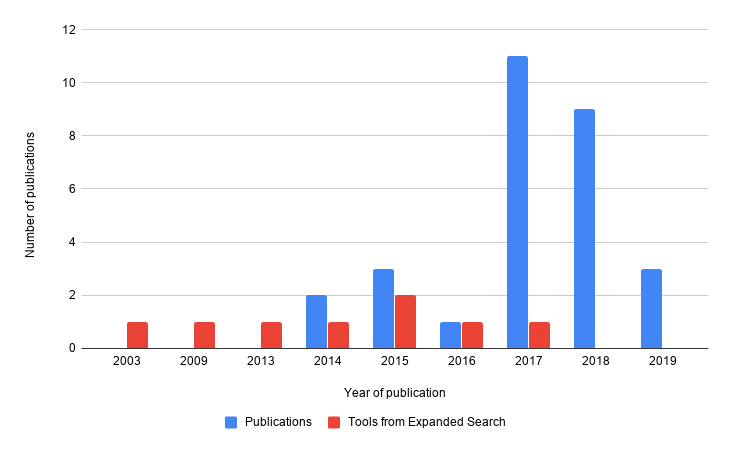
\includegraphics[width=1\textwidth]{slr_evolution.png}
\end{figure}

\subsubsection{Result Analysis}\label{sec:result_analysis}

\begin{description}
    \item [Scope] Most of the tools found have several scopes, such as education, industry or home automation. From the 28 tools, 6 were specific to Home Automation, 4 to Education, 3 to specific domains, 1 for industry and the remainder had a wide range of use cases.
    \item [Architecture] From the 28 tools found, 16 tools have a centralized architecture, 3 are decentralized and the remaining 9 didn't have enough information to reach a conclusion.
    \item [License] Most of the tools didn't mention a license and the ones who did were in its majority open source (e.g. GNU GPL2, GNU GPL3, Apache 2.0 and LGPL3). 
    \item [Tier] From the 28 tools, 9 didn't specify the tier they are situated in. From the remaining 19, 14 are situated in the Cloud layer, 3 are in the Fog and/or Edge and the remaining 2 are work both in the Cloud and Edge tiers.
    \item [Scalability] The majority of tools analyzed don't have scalability metrics analyzed, more specifically the number of devices supported by them. The ones that do have high scalability, which concludes that that result is analyzed when the tool has support for it.
    \item [Programming] From the 28 analyzed tools, 22 employ a hybrid text and visual system visual programming paradigm, while 3 use a purely visual and the other 3 a form-based one. 
    \item [Web-based] The majority of tools analyzed are web-based, being accessible with the use of a browser. Only one tool didn't provide an environment, only a specification of a visual programming language.
\end{description}

\subsubsection{Research Questions}\label{sec:answer_slr_research_questions}

The research questions presented in Section \ref{sec:slr_research_questions} served as a way of directing the research of this Systematic Literature Review and obtain answers to relevant questions regarding the available tools that apply visual programming languages to the IoT domain. These answers are:

\begin{description}
    \item [SRQ1: What relevant VPLs applied to IoT orchestration exist?] From the analyzed tools in Section \ref{sec:slr_results} and \ref{sec:slr_expanded_research}, there are around 28 visual programming tools applied to IoT orchestration. 
    \item [SRQ2: What is the tier and architecture of the tools found in RQ1?] Tables \ref{tab:slr_table_results} and \ref{tab:expanded_research_results} give an overview of the characteristics of all the tools found. In these tables and subsequent analysis in Section \ref{sec:result_analysis} it is concluded that the majority of the tools have a centralized architecture and work in the Cloud tier.
    \item [SRQ3: What was the evolution of VPLs applied to IoT orchestration over the years?] As it can be observed in Section \ref{sec:articles_nr_analysis} and more specifically in Figure \ref{fig:slr_evolution}, there are visual programming tools applied to the orchestration of IoT since 2003, and in 2017 and 2018 there was a bigger number of publications with a focus on building these type of tools.  
\end{description}


\subsection{Conclusions}\label{sec:slr_conclusions}

In this Systematic Literature Review, 2698 publications were analyzed from IEEE, ACM and Scopus databases. This resulted in 21 visual programming tools applied to the Internet-of-Things. A survey made on VPLs applied to IoT found during the research process resulted in 8 more tools, making a total of 29.

The results show that there is a significant number of tools that allow its end-users to build IoT systems using visual programming, in several different scopes. The majority of these tools have a centralized architecture and operate in the Cloud layer. Despite the good amount of tools, most of them don't have their source code accessible nor have a license. The results from the expanded search are more positive in this aspect, with the majority of them being open-source, such as Node-RED~\cite{node_red}, NETLab Toolkit~\cite{netlabtoolkit} and others. However, this poses a problem, since there is a clear lack of open source tools.

In summary, the majority of tools found don't possess a license, employ a centralized architecture, operate in the Cloud tier and use a hybrid text and visual programming system. This propels the possibility of building, as future work, a visual programming tool applied to IoT that is (1)~open-source, (2)~has a decentralized architecture and (3)~also operates in the Fog and/or Edge layers.

\section{Decentralized Architectures in Visual Programming Tools applied to the Internet-of-Things paradigm}\label{sec:sota_decentralized}


Section \ref{sec:slr} mentions some tools that aim to offer a decentralized solution to visual programming environments applied to Internet-of-Things systems~\cite{ddf}~\cite{ddflow}~\cite{wotflow_dnr}.

\subsection{DDF}\label{sec:decentralized_sota_ddf}

The work made by in WoTFlow~\cite{wotflow_dnr}, DDF~\cite{ddf} and subsequent works~\cite{fog_at_the_edge}~\cite{exogenous_coordination} consists of a system built on the Node-RED framework and focused on the use case of Smart Cities. Their goal is to make a tool more suitable for the development of fog-based applications that are dependent on the context of the edge devices they operate on. 

In DDF~\cite{ddf}, they started by extending Node-RED and implementing D-NR (Distributed Node-RED), which contains processes that can run across devices in local networks and servers in the Cloud. The application, called flow, is built in the visual programming environment, which is running in a development server. All the other devices running D-NR subscribe to an MQTT topic that contains the status of the flow. When a flow is deployed, all devices running D-NR are notified and subsequently analyze the given flow. Based on a set of constraints, they decide which nodes they may need to deploy locally and which sub-flow (parts of a flow) must be shared with other devices. Each device has a set of characteristics, from its computational resources such as bandwidth, available storage to its location. The developer can insert constraints into the flow, by specifying which device a sub-flow must be deployed in or the computational resources needed. However, these constraints and the characteristics of each device must be manually inserted in the system by developers or system operators. 

Subsequent work to the previously mentioned tool focused on support for the Smart Cities domain. In the publication of 2018~\cite{fog_at_the_edge}, the problems addressed were the deployment of multiple instances of devices running the same sub-flow was a developed feature, as well as the support for more complex deployment constraints of the application flow. With this, the developer can specify requirements for each node on device identification, computing resources needed (CPU and memory) and physical location. In addition to these improvements, the coordination between nodes in the fog was tackled by introducing a coordinator node. This node is responsible for synchronizing the context of the device with the one given by the centralized coordinator. In Figure \ref{fig:coordination_dnr} it is possible to see the four possible states of a coordinator node: (1)~NORMAL, where the node passes the data to its output, (2)~DROP, in which the node does not pass the data to other node and instead drops it, (3)~FETCH\_FORWARD, where the node gets the input from an external instance of its supposed input and (4)~RECEIVE\_REDIRECT in which the node sends the data to an external instance of its output node.

In more recent work~\cite{exogenous_coordination}, support for CPSCN (Cyber-Physical Social Computing and Networking) was implemented, making it possible to facilitate the development of large scale CPSCN applications. To make this possible, the contextual data and application data were separated, so that the application data is only used for computation activities and the contextual data is used to coordinate the communication between those activities.

\begin{figure}[h]
\caption{Coordination between nodes in D-NR~\cite{fog_at_the_edge}}
\label{fig:coordination_dnr}
\centering
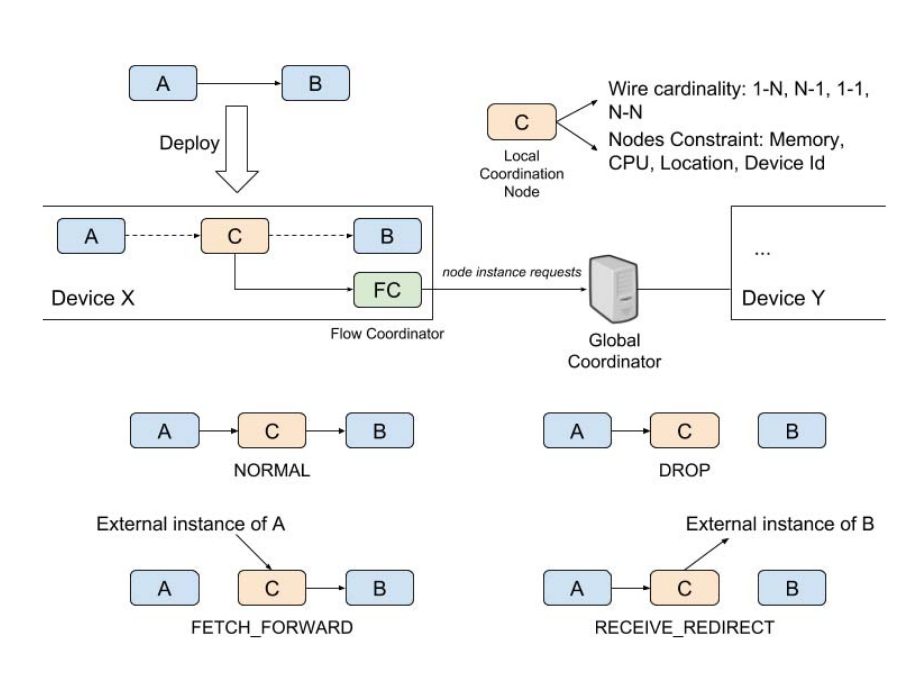
\includegraphics[width=0.8\textwidth]{dnr_exogenous_coordination.png}
\end{figure}

\subsection{\textit{FogFlow \& uFlow}}\label{sec:decentralized_sota_uflow}

Another approach was made in the publication by Szydlo et al.~\cite{flow_based_programming_fog}, where they focused on the transformation and decomposition of data flow. Parts of the flow can be translated into the executable parts, such as Lua code. Their contribution includes the concepts of data flow transformation, a new run-time environment called \textit{uFlow} that can be executed on a variety of resource-constrained embedded devices and the integration with the Node-RED platform. 

The solution found consisted of the transformation of a given data flow, where the developer chooses the computing operations that will be run on the devices. The operations that will run directly on the devices are implemented in the form of embedded software, using the developed framework \textit{uFlow}, which allows for parts of the flow to be run on heterogeneous devices. All this is integrated with Node-RED. The communication between the devices is made only through the cloud, with no support for peer-to-device communication. The results were promising, with a decrease in the number of measurements made by the sensors. However, there was room for improvement, with the automation of the decomposition and partitioning of the initial flow, the detection bottlenecks which will move computations accordingly from the cloud to the fog. Figure \ref{fig:uflow_1} represents a situation of partitioning and assignment of tasks. There are two IoT devices and a Node-RED instance running in the Cloud. The system's goal is to measure soil humidity and ambient light. If a button is pressed or fertilizer is needed, an e-mail is sent to the gardener. The partition of computation is made in the assumption that the closer a selected process it to the source of data, the higher the amount of data transmitted between computing operations. After parts of the flow are assigned to specific devices, they are altered in order to be executed by \textit{uFlow} and Node-RED. It is possible to observe in Figure \ref{fig:uflow_1} the results of the transformation process, where the parts of the flow surrounded by color are executed in the device with the respective color.

\begin{figure}[h]
\caption{Partition and assignment of parts of the flow \cite{flow_based_programming_fog}}
\label{fig:uflow_1}
\centering
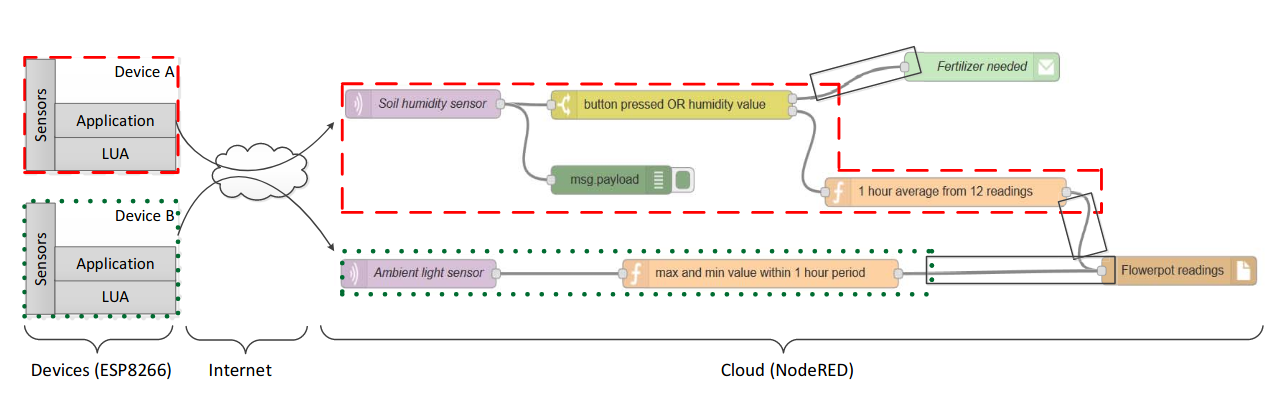
\includegraphics[width=0.9\textwidth]{uflow_1.png}
\end{figure}

In 2019, they continued their work with the publication~\cite{fog_flow}, where they built the model and engine \textit{FogFlow}, which enables the design of applications able to be decomposed onto heterogeneous IoT environments according to a chosen decomposition schema. To achieve a level of decentralization and heterogeneity, they abstract out the application definition from its architecture and rely on graph representation to provide an unambiguous, well-defined model of computations. The application definition should be infrastructure-independent and contain only data processing logic, and its execution should be possible on different sets of devices with different capabilities. Several algorithms for flow decomposition were mentioned~\cite{algorithm_fog}~\cite{ifogsim}, but none were specified in terms of results. Figure \ref{fig:fogflow} represents the \textit{FogFlow} architecture, which is composed by three modules: (1)~the \textit{FogFlow} API, which enables the creation of the application definition, (2)~the Graph Module, responsible for processing and transforming the application definition into a data flow graph and finally the (3)~Execution Model, which translates the graph and generates executables ready to be run on the assigned devices.

\begin{figure}[h]
\caption{\textit{FogFlow} architecture \cite{fog_flow}}
\label{fig:fogflow}
\centering
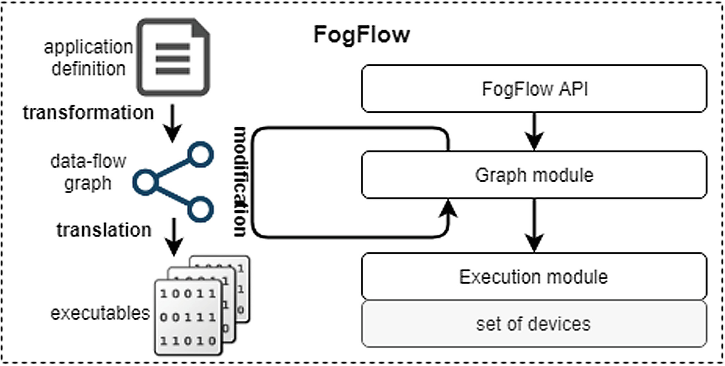
\includegraphics[width=0.8\textwidth]{fogflow.png}
\end{figure}

\subsection{\textit{FogFlow}}\label{sec:decentralized_sota_fogflow}

There is another tool with the same name \textit{FogFlow} but created by Cheng et al.~\cite{fogflow_github}. In the first publication related to this tool~\cite{fog_flow_easy}, the contributions made were the implementation of a standards-based programming model for Fog Computing and scalable context management. The first contribution consists in extending the dataflow programming model with hints to facilitate the development of fog applications. The scalable context management introduces a distributed approach, which allows overcoming the limits in a centralized context, achieving much better performance in terms of throughput, response time and scalability. The \textit{FogFlow} framework focuses in a Smart City Platform use case, separated in three areas: (1)~Service Management, normally hosted in the cloud, (2)~Data Processing, present in cloud and edge devices and (3)~Context Management, which is separated in an device discovery unit hosted in the cloud and IoT brokers scattered in edge and cloud.

In more recent work~\cite{fog_flow_tool}, \textit{FogFlow} was improved to provide infrastructure providers with an environment that allows them to build decentralized IoT systems faster, with increased stability and scalability. The architecture can be seen in Figure \ref{fig:fogflow_tool}, where the IoT system is represented by dynamic data flows that are orchestrated between sensors (Producers) and actuators (Consumers). The application is first designed using the \textit{FogFlow} Task Designer, a hybrid text and visual programming environment, which results in an abstraction called Service Template. This abstraction contains specifics about the resources needed for each part of the system. Once the Service Template is submitted, the framework will determine how to instantiate it using the context data available. Each task is associated with an operator, which consists of a Docker image, and its assignment is based on how many resources are available on each edge node, the location of data sources and the prediction of workload. Edge nodes are autonomous since they can make their own decisions based on their local context, without relying on the central cloud.

\begin{figure}[h]
\caption{\textit{FogFlow} high level model~\cite{fog_flow_tool}}
\label{fig:fogflow_tool}
\centering
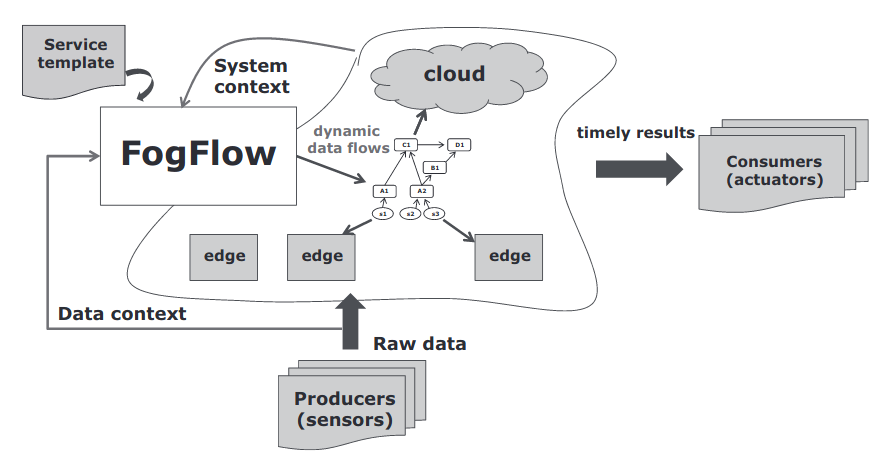
\includegraphics[width=0.8\textwidth]{fogflow_tool.png}
\end{figure}

\subsection{DDFlow}\label{sec:decentralized_sota_ddflow}

DDFlow~\cite{ddflow}, first mentioned in Section \ref{sec:slr_results}, presents another distributed approach by extending Node-RED with a system run-time that supports dynamic scaling and adaption of application deployments. The coordinator of the distributed system maintains the state and assigns tasks to available devices, minimizing end-to-end latency. Dataflow notions of \textit{node} and \textit{wire} are expanded, with a \textit{node} in DDFlow representing an instantiation of a task that is deployed in a device, receiving inputs and generating outputs. \textit{Nodes} can be constrained in their assignment by optional parameters, \textit{Device}, and \textit{Region}, inserted by the developer. A \textit{wire} connects two or more nodes and can have three types: \textit{Stream} (one-to-one), \textit{Broadcast} (one-to-many) and \textit{Unite} (many-to-one). 

In a DDFlow system, each device has a set of capabilities and a list of services that correspond to an implementation of a \textit{Node}, as can be seen in Figure \ref{fig:ddflow}. The devices communicate this information through their Device Manager or a proxy, if it is a constrained device. The Coordinator is a web server responsible for managing the DDFlow applications and is composed of three parts, which can be seen in Figure \ref{fig:ddflow}: (1)~a visual programming environment were DDFlow application are built, (2)~a Deployment Manager that communicates with the Device Managers of the devices and (3)~a Placement Solver, responsible for decomposing and assigning tasks to the available devices. When an application is deployed, a network topology graph and a task graph are constructed based on the real-time information retrieved from the devices. The Coordinator proceeds with mapping tasks to devices by minimizing the task graph's end-to-end latency of the longest path. Dynamic adaptation is supported by monitoring the system and adapting to changes. If changes in the network are detected, such as the failure or disconnection of a device, adjustments in the assignment of tasks are made. In addition to this, the Coordinator can be replicated onto many devices to improve the reliability and fault-tolerance of the system.

In the evaluation made to DDFlow, the system is able to recover from network degradation or device overload, whereas in a centralized system this would cause its total failure.

\begin{figure}[h]
\caption{DDFlow architecture}
\label{fig:ddflow}
\centering
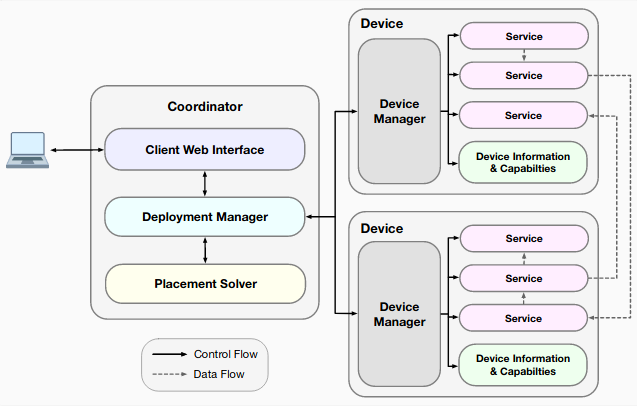
\includegraphics[width=0.8\textwidth]{ddflow.png}
\end{figure}

\subsection{Conclusions}\label{sec:decentralized_sota_conclusions}

From the tools analyzed, it can be concluded that the state of the art in decentralized architectures in visual programming tools applied to IoT is incomplete. All the tools leverage the devices in the network but in different ways. DFF~\cite{ddf} assumes that all devices run Node-RED, which limits the type of devices that can be leveraged since it needs to have minimum resources to run it. \textit{FogFlow} and \textit{uFlow}~\cite{fog_flow}~\cite{flow_based_programming_fog} is the only tool that specifies how it truly leverages constrained devices, with the transformation of sub-flows into Lua code, with DDFlow~\cite{ddflow} assuming that all devices have a list of specific services they can provide, that should match the node assigned to them.

Regarding the method used to decompose and assign computations to the available devices, DDFlow describes the process with the use of a longest path algorithm focused on reducing end-to-end latency between devices. \textit{FogFlow} and \textit{uFlow}~\cite{fog_flow}~\cite{flow_based_programming_fog} mention several algorithms that could be used, but don't specify which one was implemented. Both DDF~\cite{ddf} and \textit{FogFlow}~\cite{fog_flow_easy}~\cite{fog_flow_tool} don't specify the algorithm used besides some constraints but are the only tools with their source code accessible and with an open-source license. All the tools claim to have support for run-time adaptation to changes in the system, such as device failures.

%\cite{mobile_cloud_heterogeneous}
%\cite{mobile_cloud}

\section{Summary}

Section \ref{sec:slr} presents a Systematic Literature Review of visual programming tools applied to the Internet-of-Things. Each tool derived from the research is summarized and characterized to understand the state of the art regarding this topic of interest. Section \ref{sec:sota_decentralized} describes visual programming tools for building IoT systems that employ a decentralized architecture, pointing out their advantages but also their shortcomings.

